\begin{figure}[!htbp]
\begin{center}
\rotatebox{90}{~~~~~Mutational Load 1}
\begin{subfigure}[b]{0.45\columnwidth}
  \centering
  Small Resource Wave\\~\\
  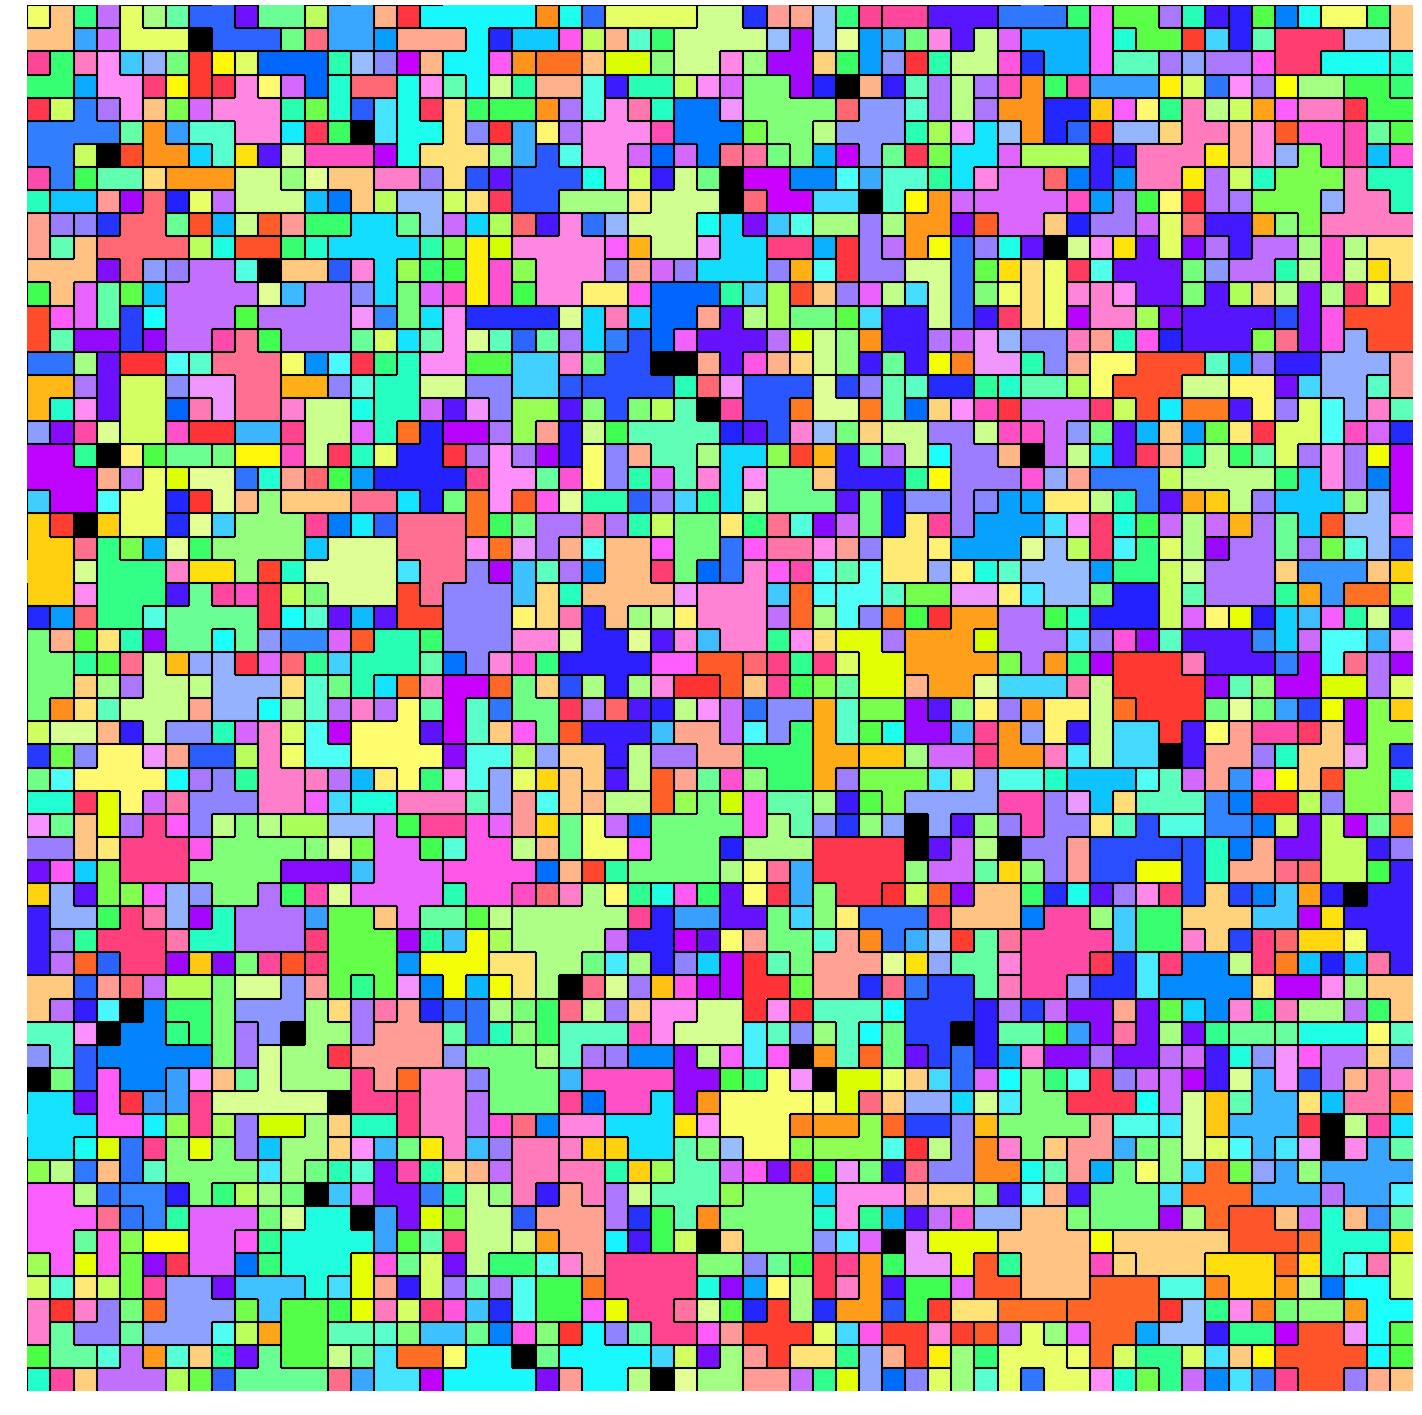
\includegraphics[width=\columnwidth]{seed=1001+title=channel_viz+treat=wave-small__mut-a_low+update=50000+_data_hathash_hash=38f284fb779ed3f5+_script_fullcat_hash=474b4115ecde8750+_source_hash=d53f428-clean+ext=}
\end{subfigure}
\begin{subfigure}[b]{0.45\columnwidth}
  \centering
  Large Resource Wave\\~\\
  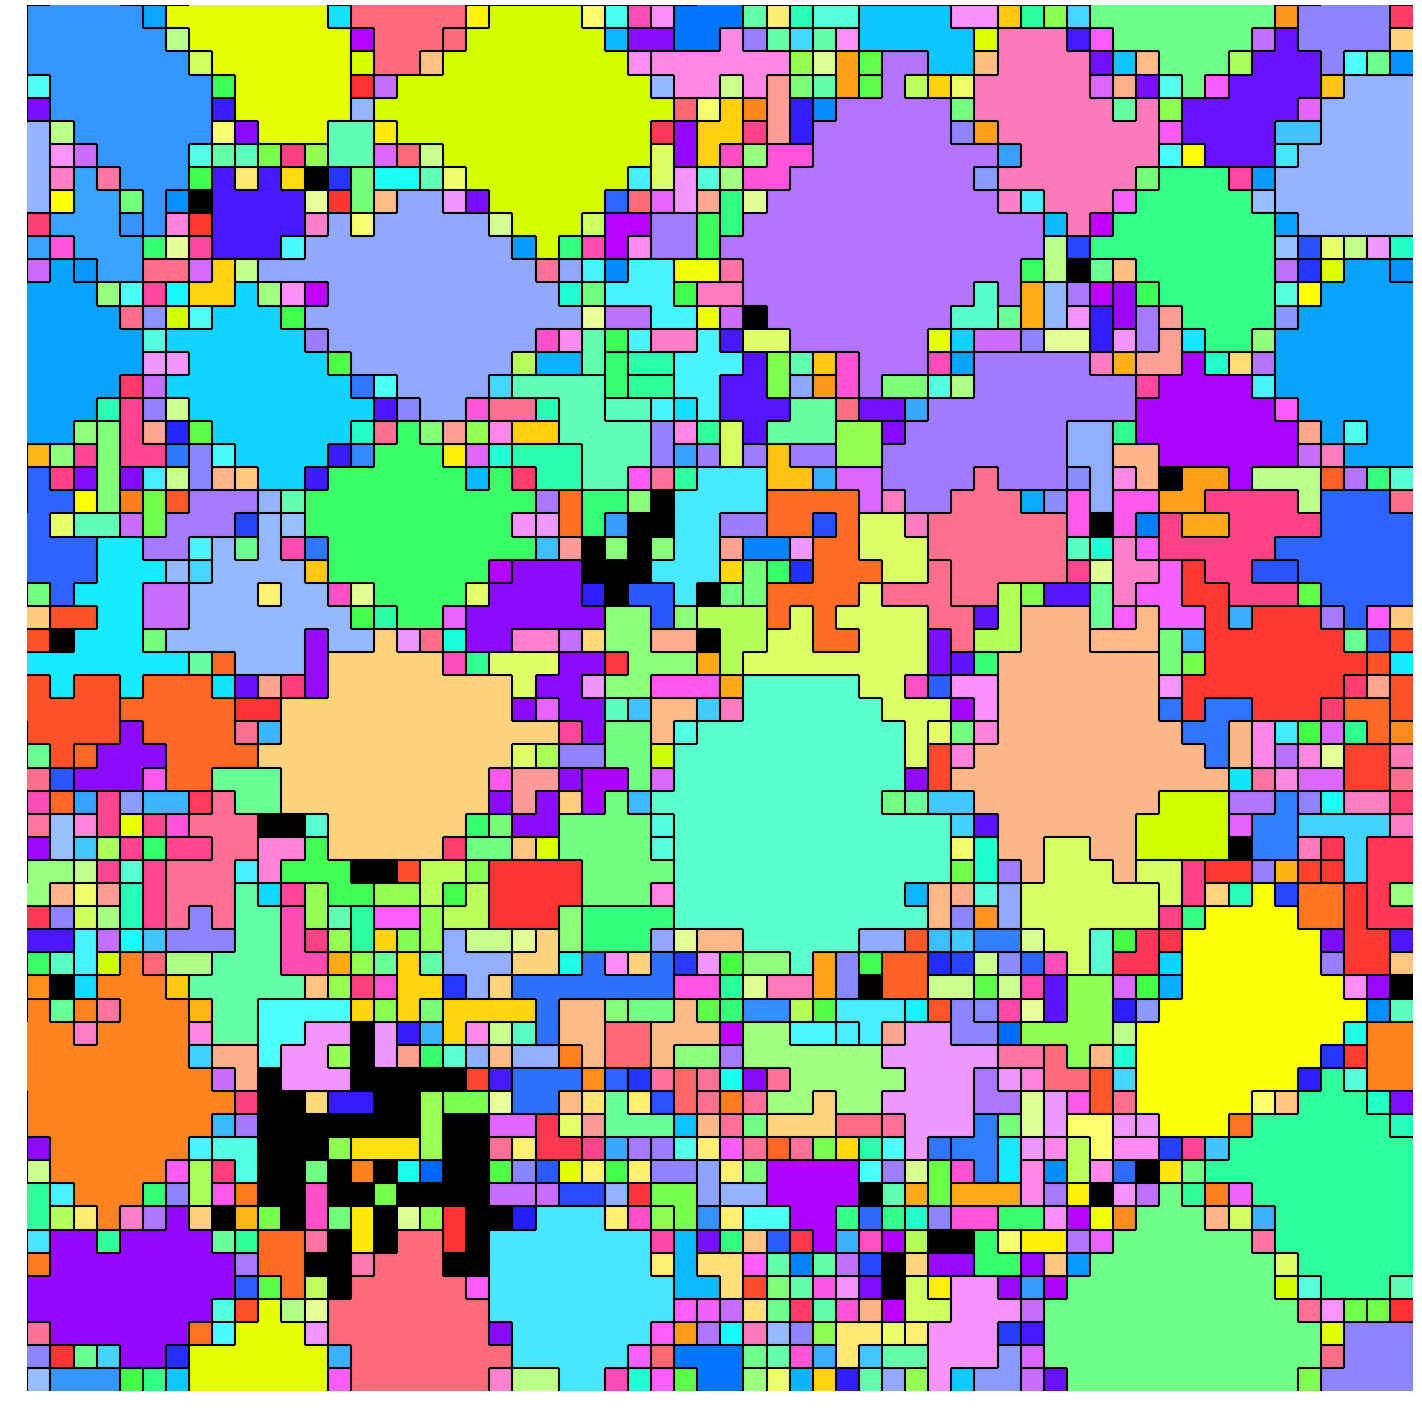
\includegraphics[width=\columnwidth]{seed=1001+title=channel_viz+treat=wave-big__mut-a_low+update=50000+_data_hathash_hash=33ac6f19e90e7ab9+_script_fullcat_hash=474b4115ecde8750+_source_hash=d53f428-clean+ext=}
\end{subfigure}

\rotatebox{90}{~~~~~~~Mutational Load 2}
\begin{subfigure}[b]{0.45\columnwidth}
  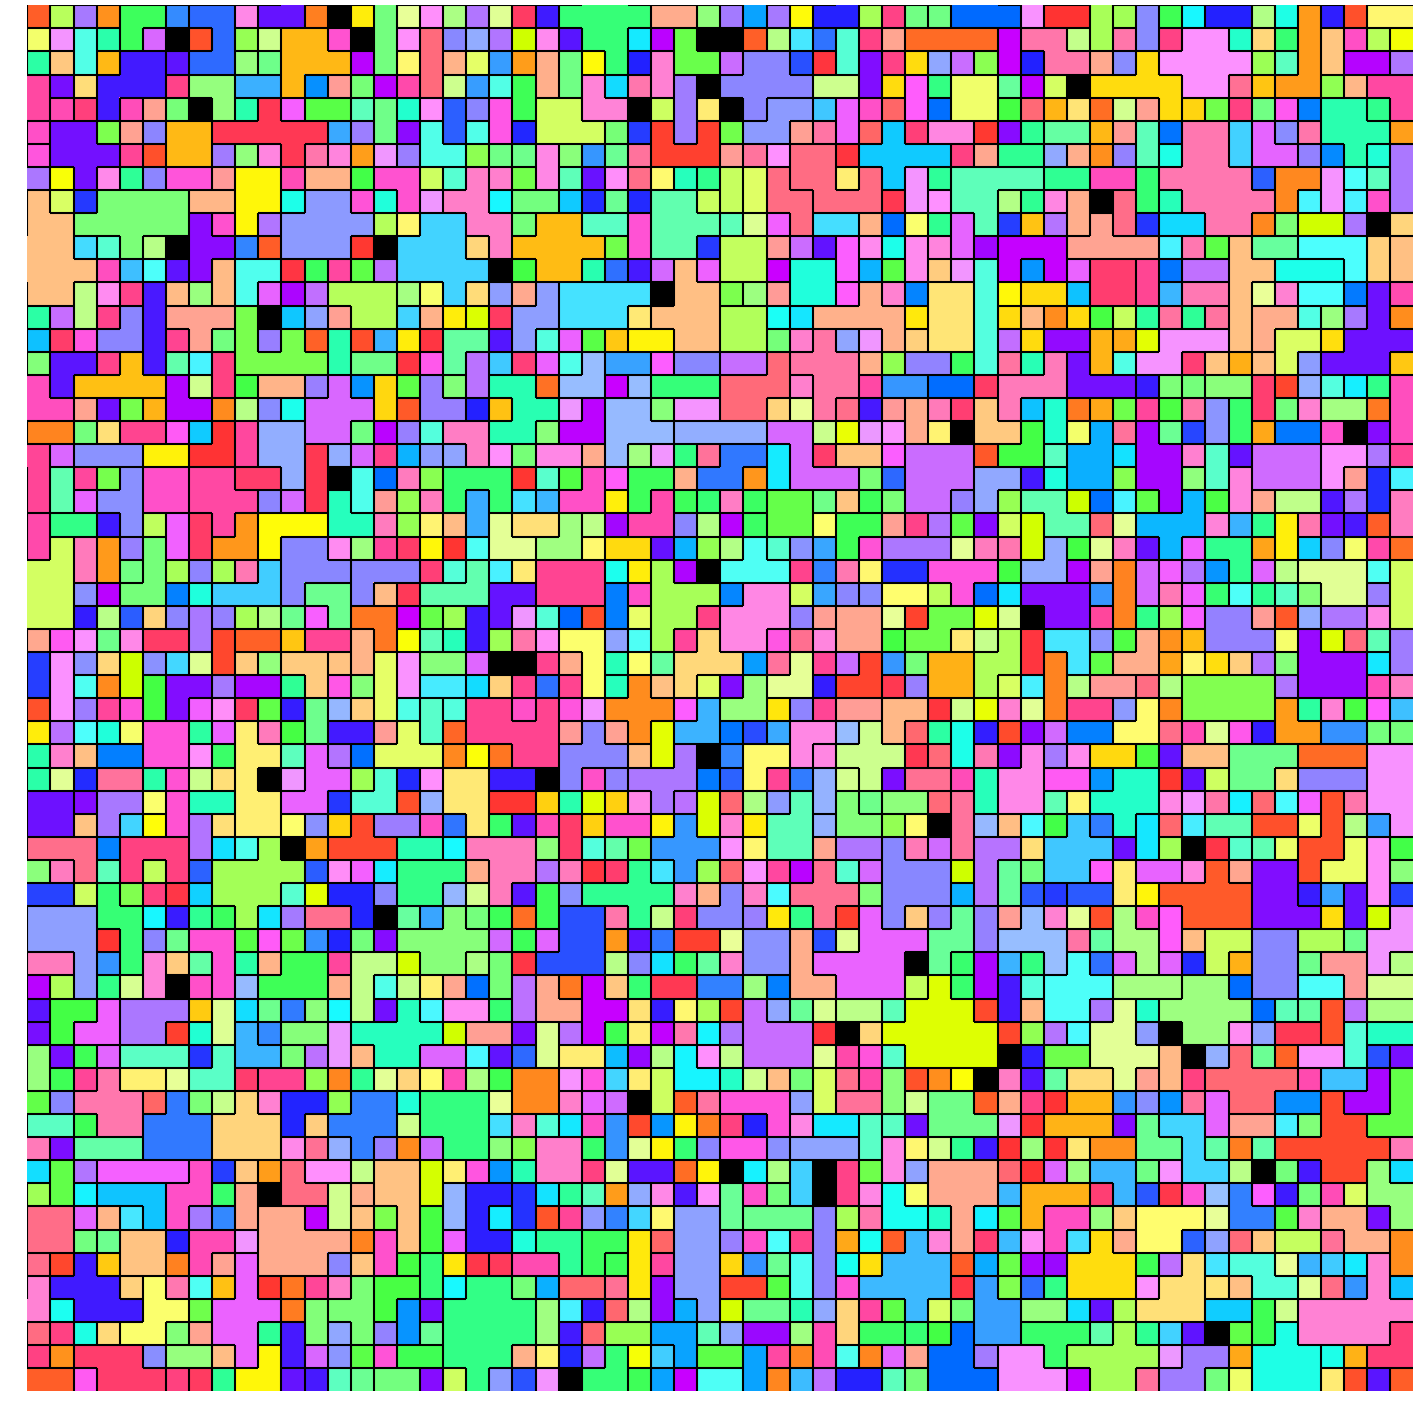
\includegraphics[width=\columnwidth]{seed=1001+title=channel_viz+treat=wave-small__mut-b_medlow+update=50000+_data_hathash_hash=0c0190afbbcd9acb+_script_fullcat_hash=474b4115ecde8750+_source_hash=d53f428-clean+ext=}
\end{subfigure}
\begin{subfigure}[b]{0.45\columnwidth}
  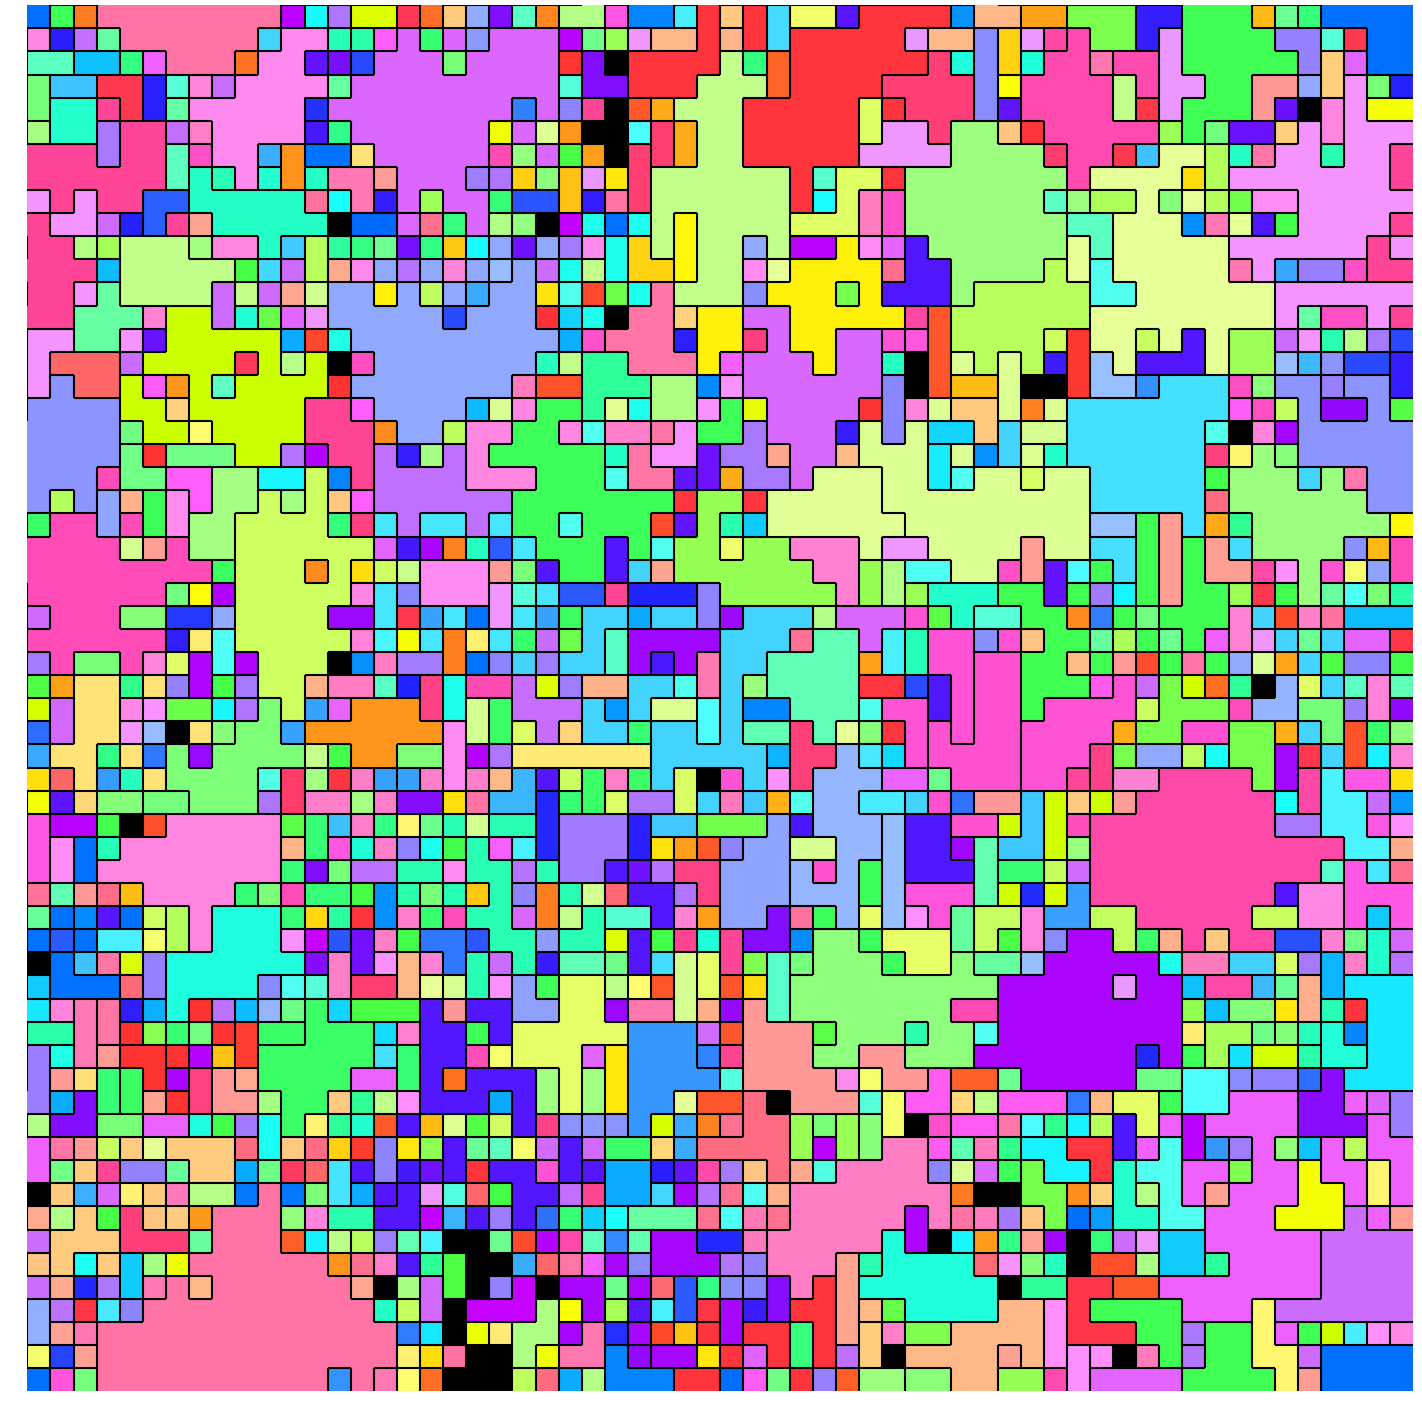
\includegraphics[width=\columnwidth]{seed=1001+title=channel_viz+treat=wave-big__mut-b_medlow+update=50000+_data_hathash_hash=50427fb0ffaf976a+_script_fullcat_hash=474b4115ecde8750+_source_hash=d53f428-clean+ext=}
\end{subfigure}

\rotatebox{90}{~~~~~~~Mutational Load 3}
\begin{subfigure}[b]{0.45\columnwidth}
  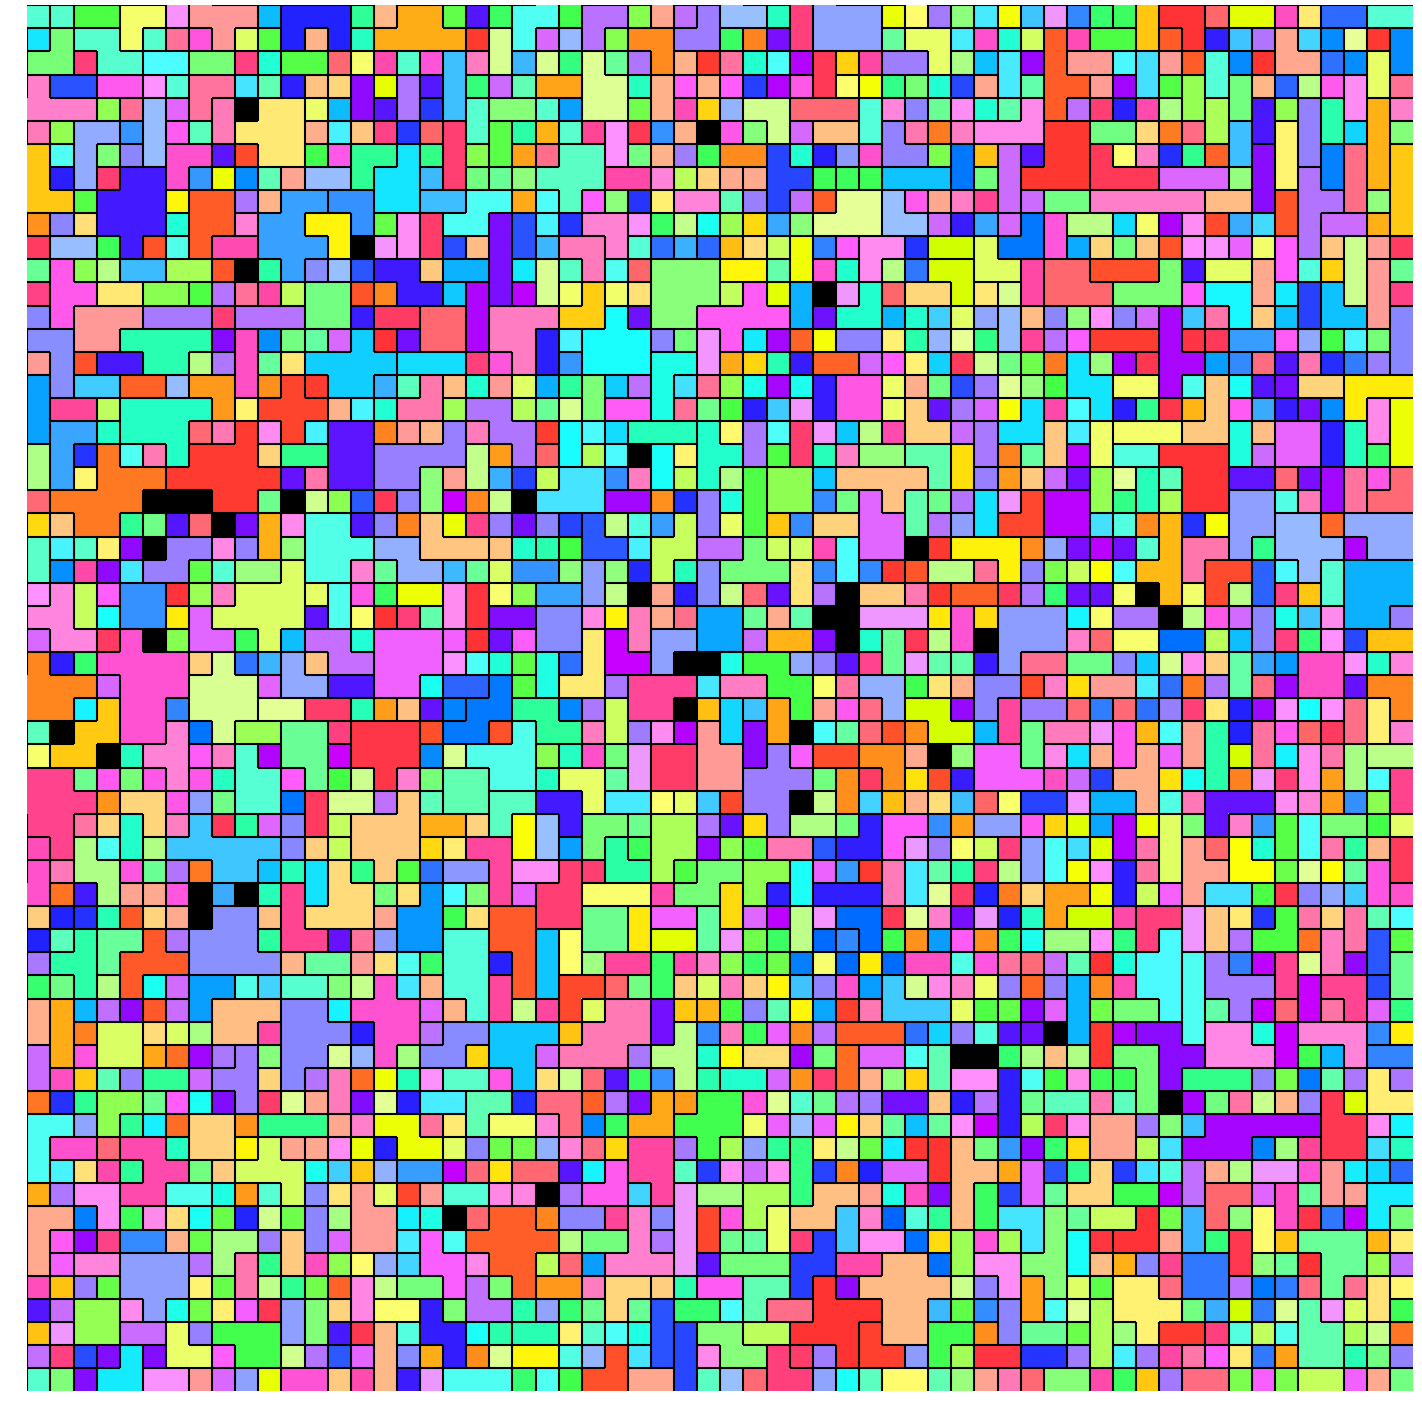
\includegraphics[width=\columnwidth]{seed=1001+title=channel_viz+treat=wave-small__mut-c_medhigh+update=50000+_data_hathash_hash=153e2f8791347e2b+_script_fullcat_hash=474b4115ecde8750+_source_hash=d53f428-clean+ext=}
\end{subfigure}
\begin{subfigure}[b]{0.45\columnwidth}
  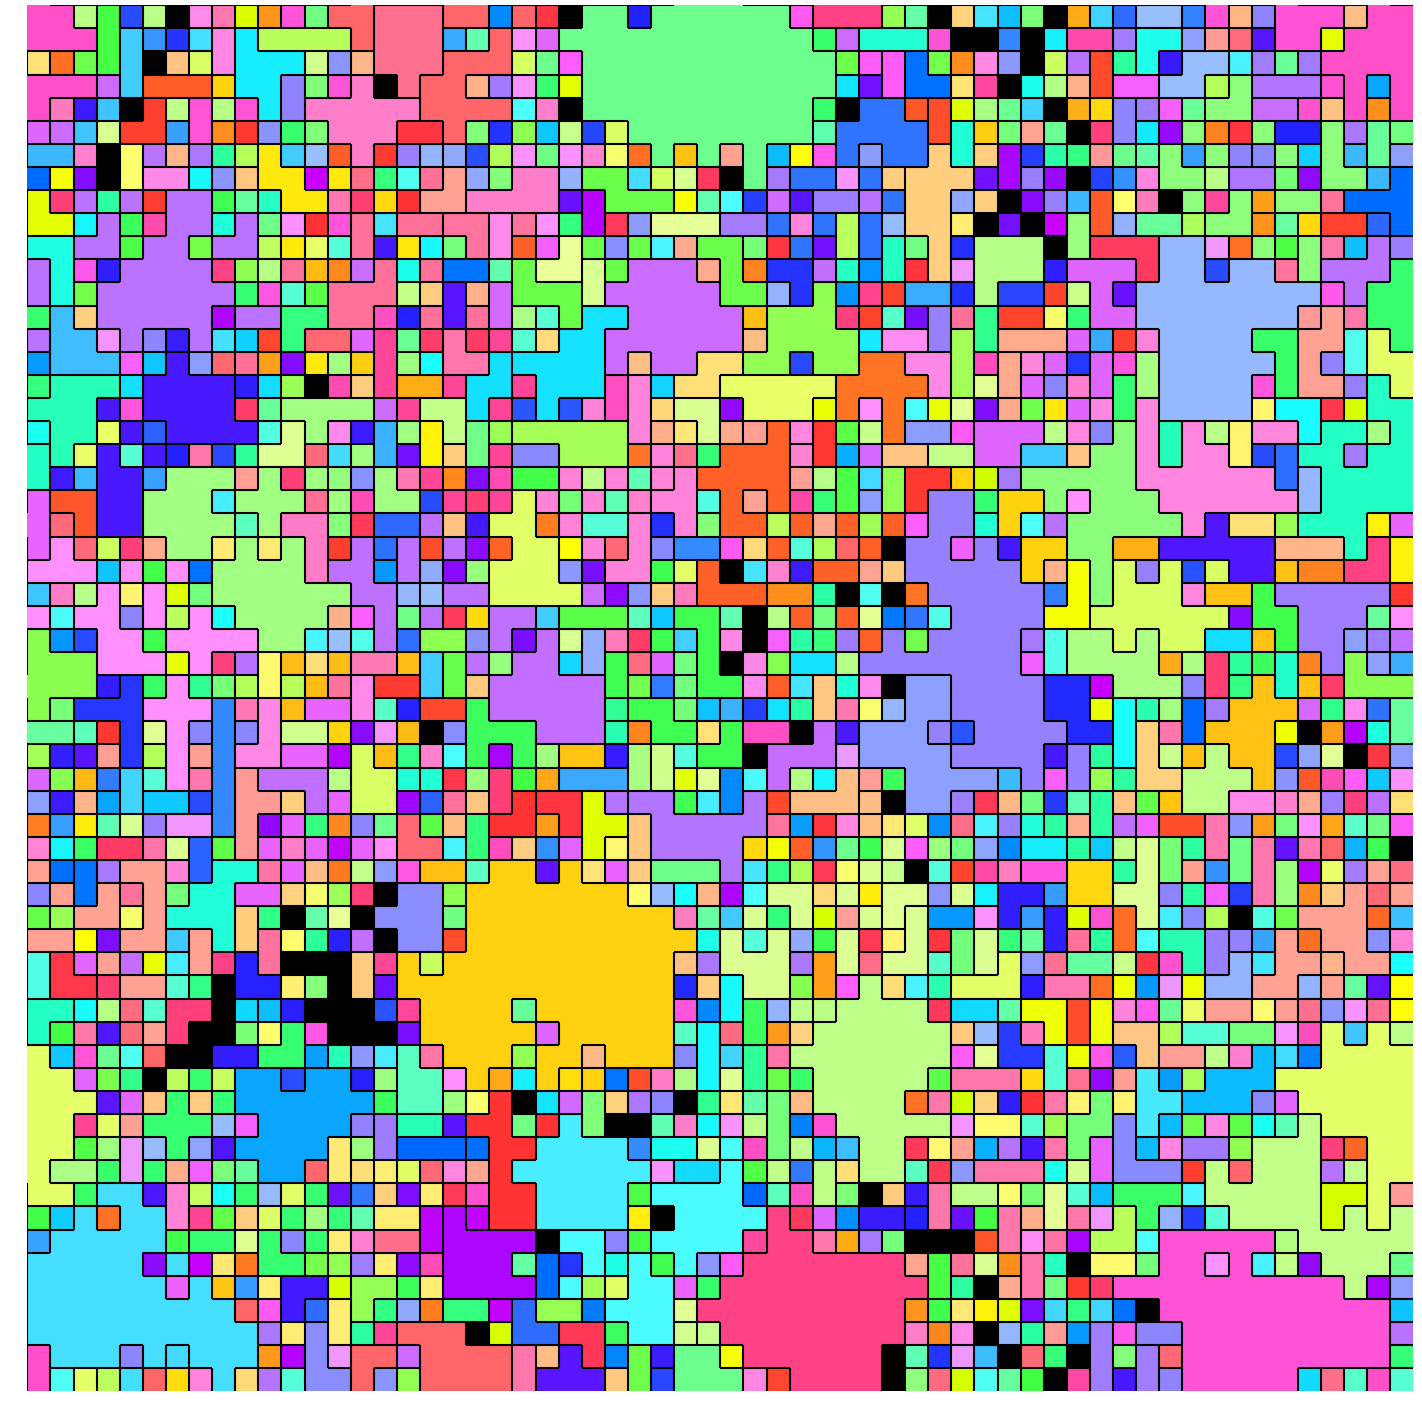
\includegraphics[width=\columnwidth]{seed=1001+title=channel_viz+treat=wave-big__mut-c_medhigh+update=50000+_data_hathash_hash=3bc8464cdb13317c+_script_fullcat_hash=474b4115ecde8750+_source_hash=d53f428-clean+ext=}
\end{subfigure}

\rotatebox{90}{~~~~~~~Mutational Load 4}
\begin{subfigure}[b]{0.45\columnwidth}
  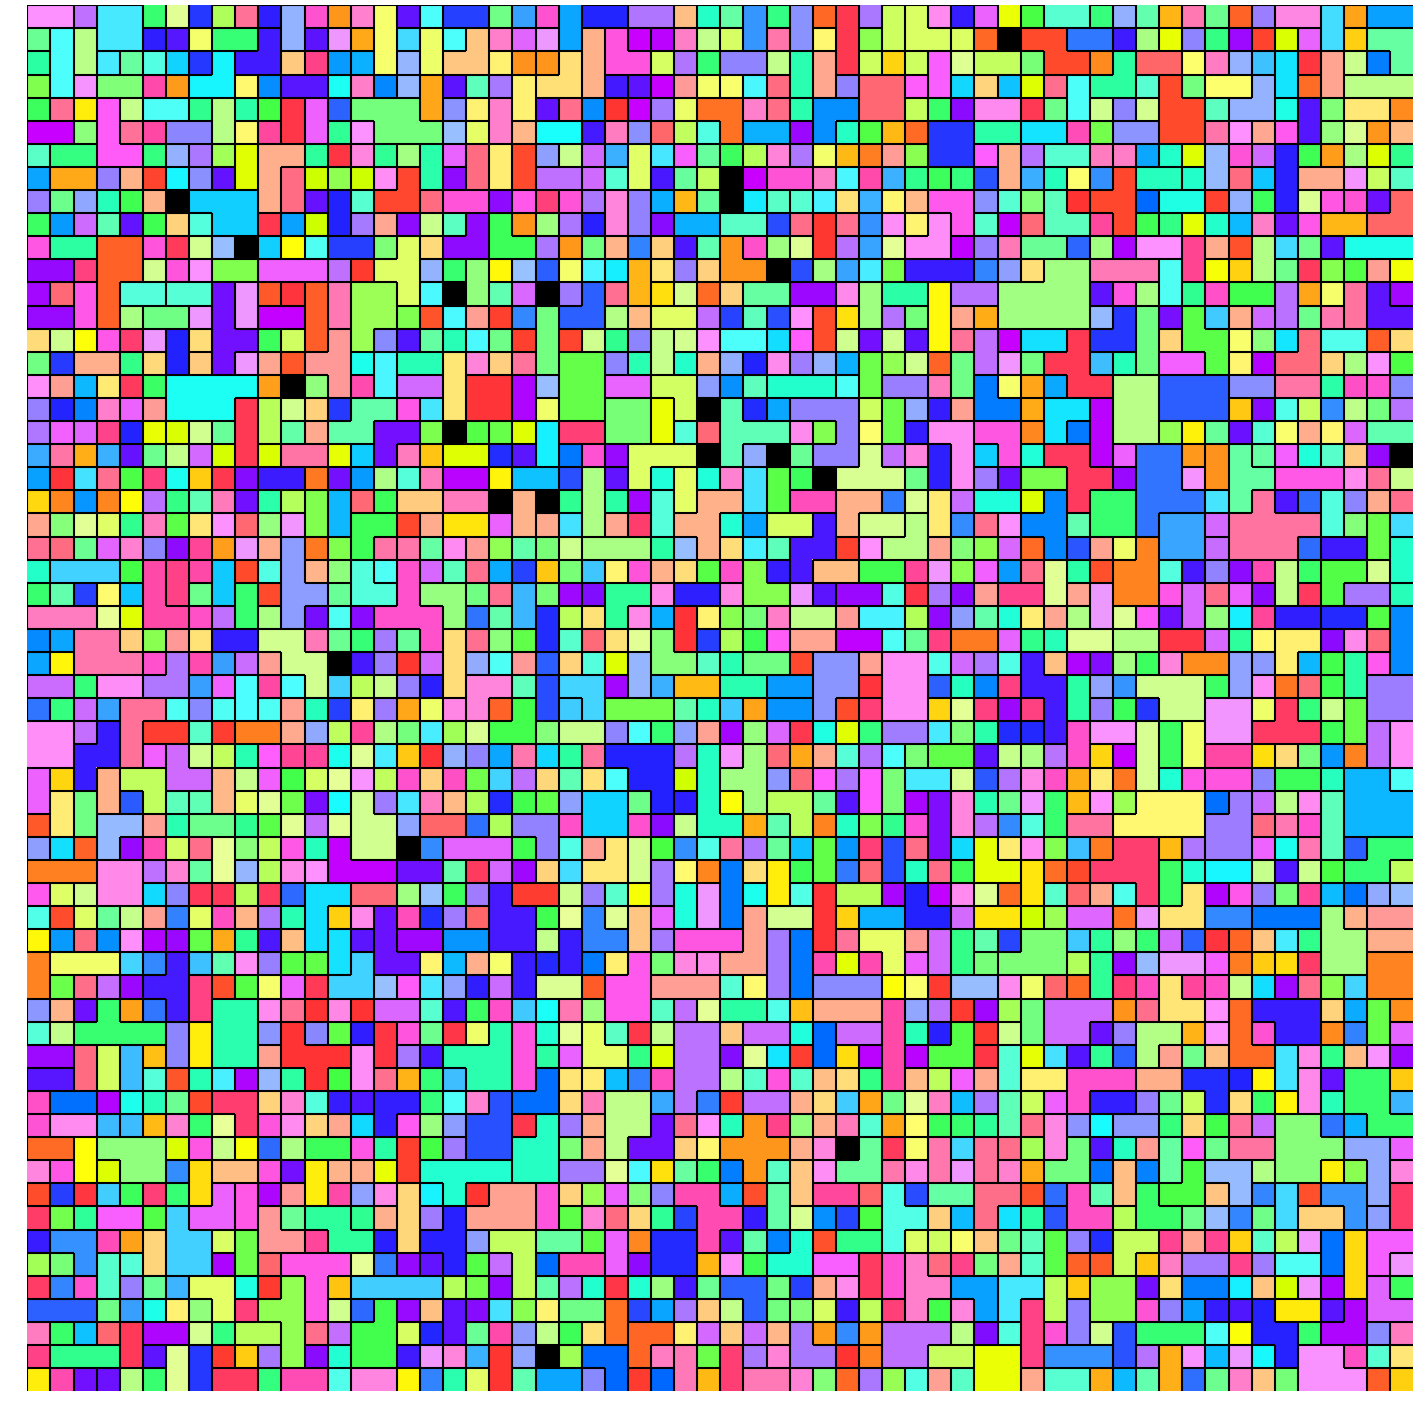
\includegraphics[width=\columnwidth]{seed=1001+title=channel_viz+treat=wave-small__mut-d_high+update=50000+_data_hathash_hash=700947e5ae80d046+_script_fullcat_hash=474b4115ecde8750+_source_hash=d53f428-clean+ext=}
\end{subfigure}
\begin{subfigure}[b]{0.45\columnwidth}
  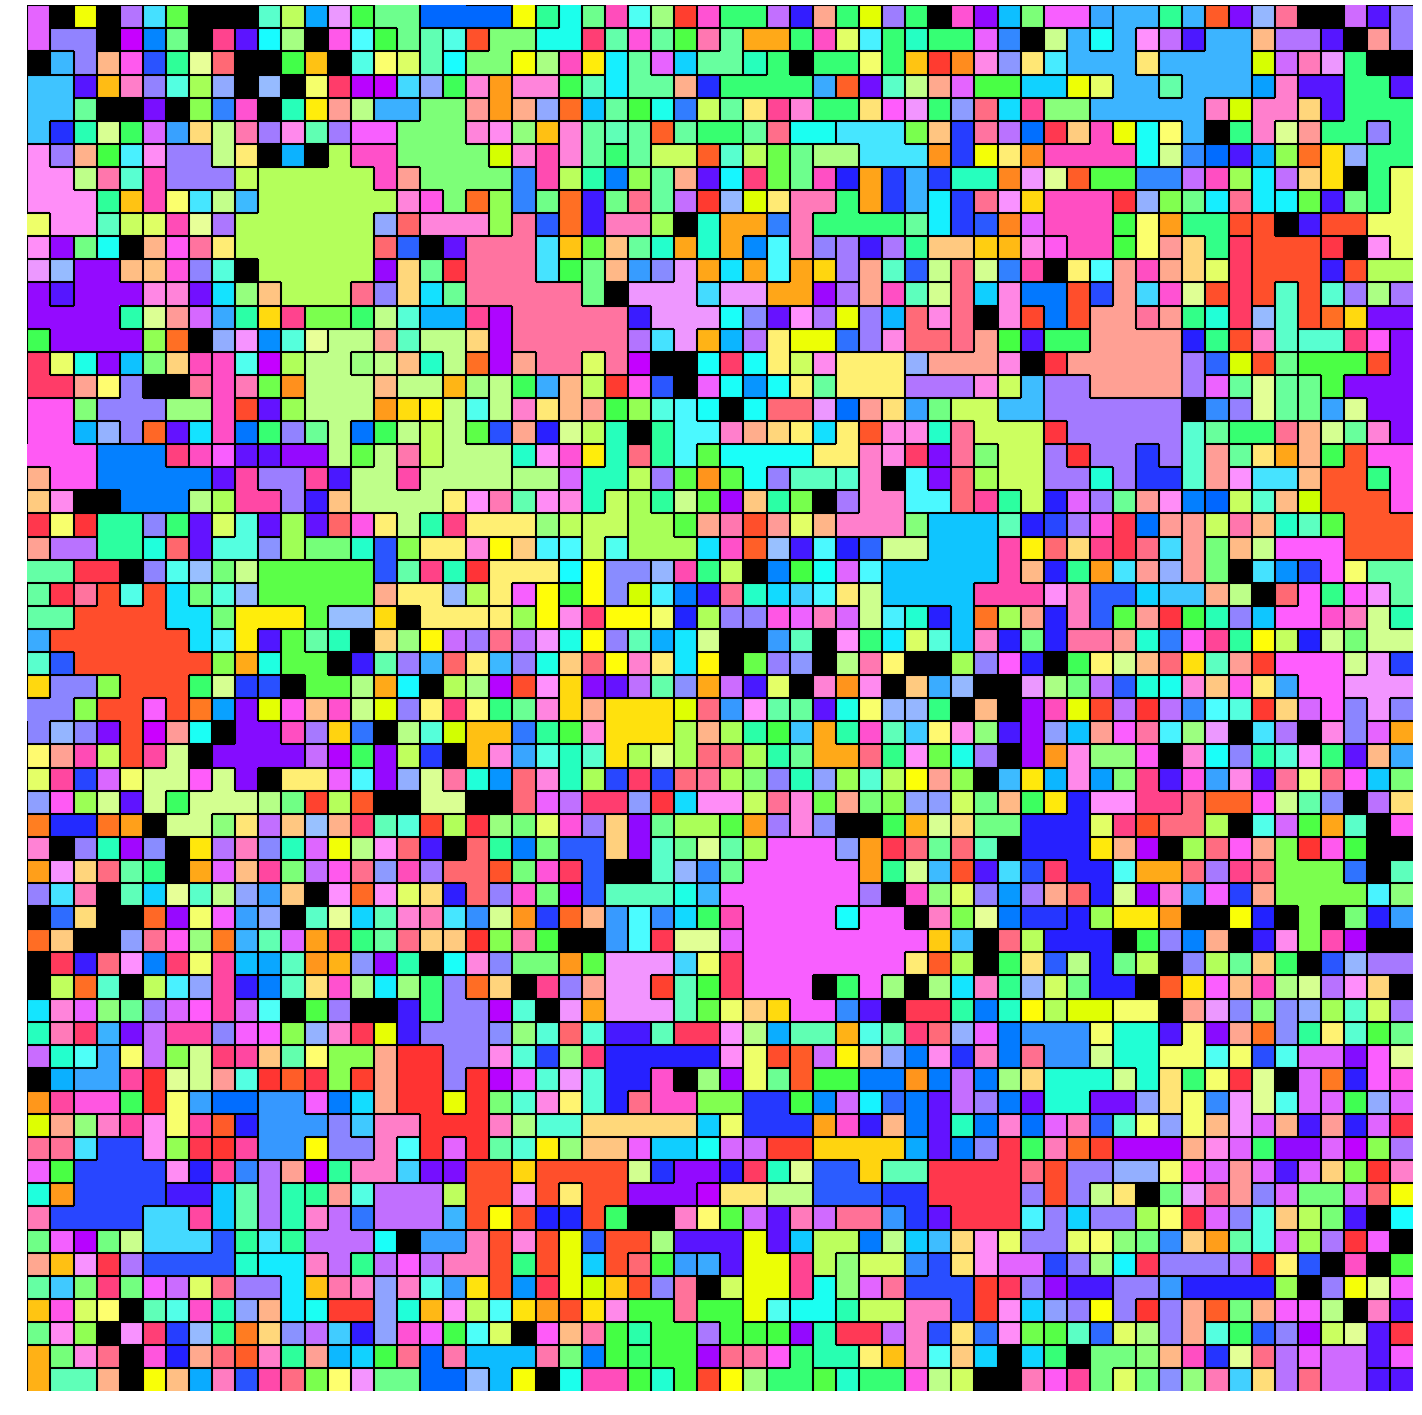
\includegraphics[width=\columnwidth]{seed=1001+title=channel_viz+treat=wave-big__mut-d_high+update=50000+_data_hathash_hash=e7071e390f076a00+_script_fullcat_hash=474b4115ecde8750+_source_hash=d53f428-clean+ext=}
\end{subfigure}

\rotatebox{90}{~~~~~~~Mutational Load 5}
\begin{subfigure}[b]{0.45\columnwidth}
  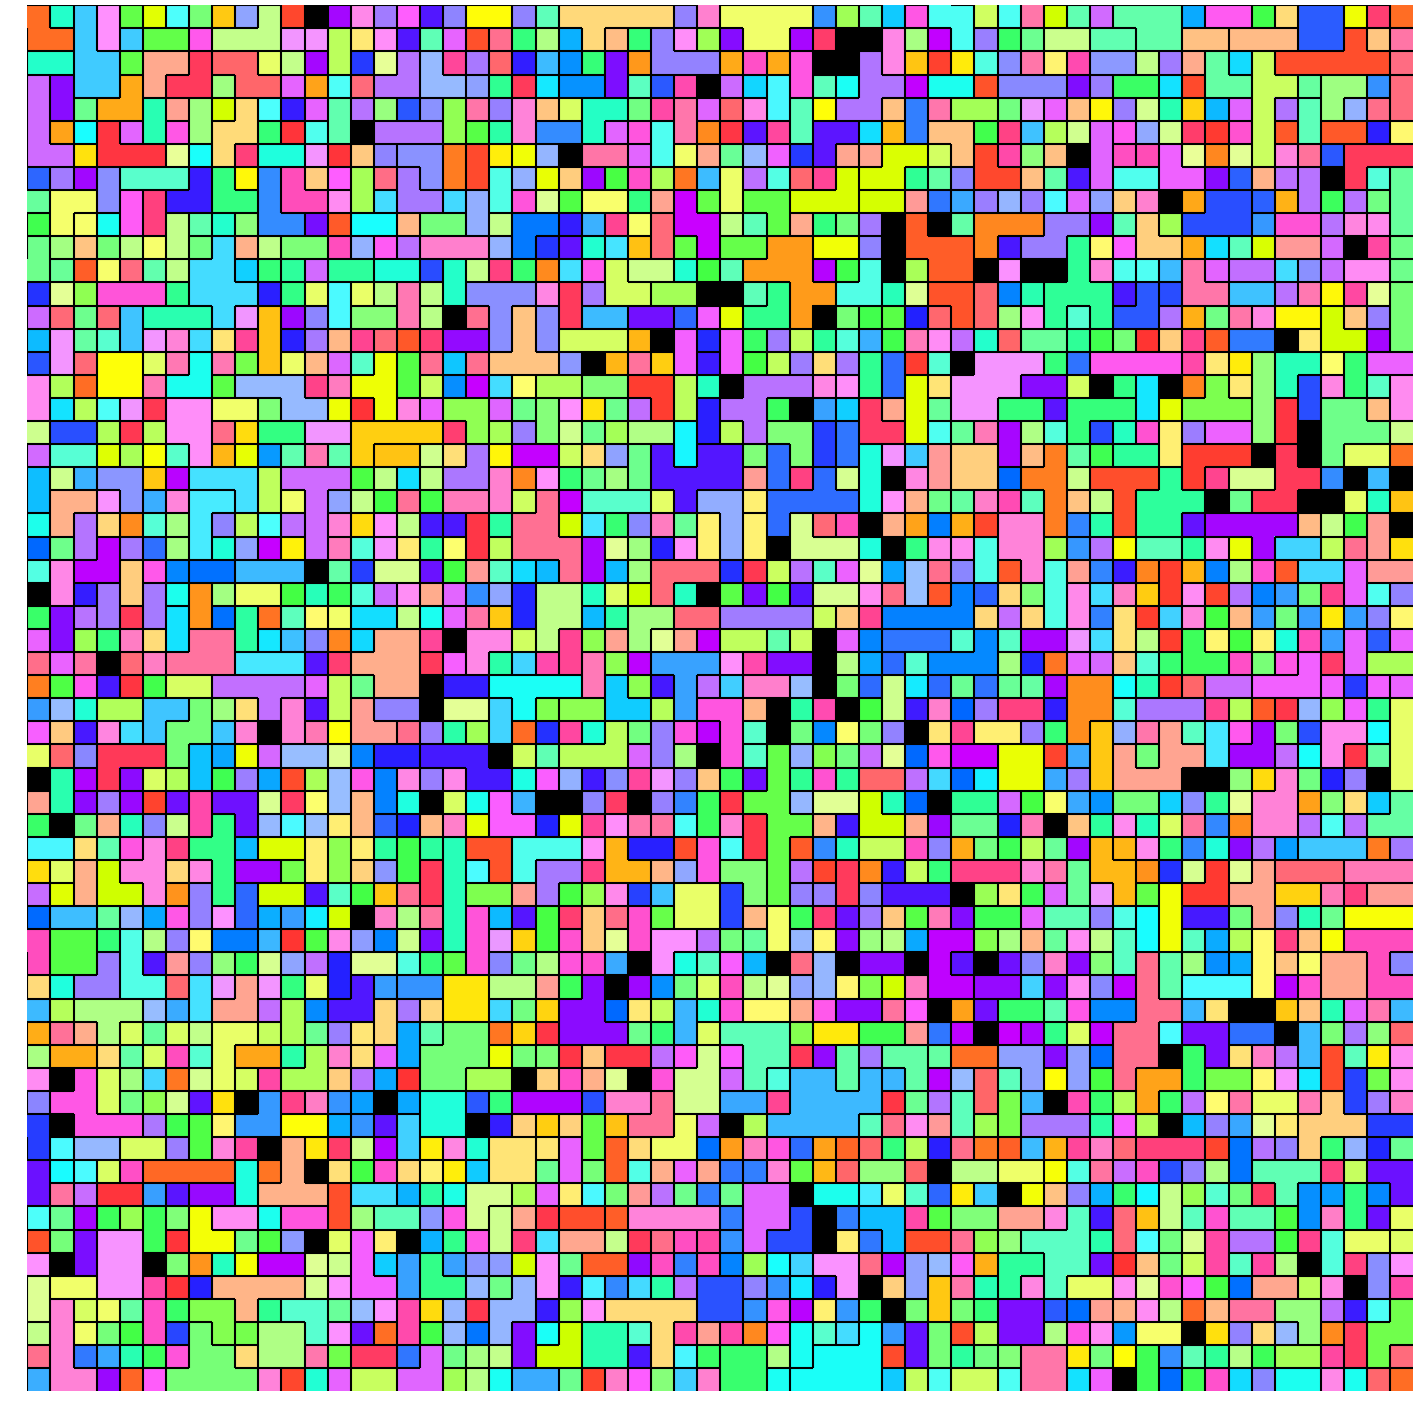
\includegraphics[width=\columnwidth]{seed=1001+title=channel_viz+treat=wave-small__mut-e_extreme+update=50000+_data_hathash_hash=70d59bcccb7f3ca6+_script_fullcat_hash=474b4115ecde8750+_source_hash=d53f428-clean+ext=}
\end{subfigure}
\begin{subfigure}[b]{0.45\columnwidth}
  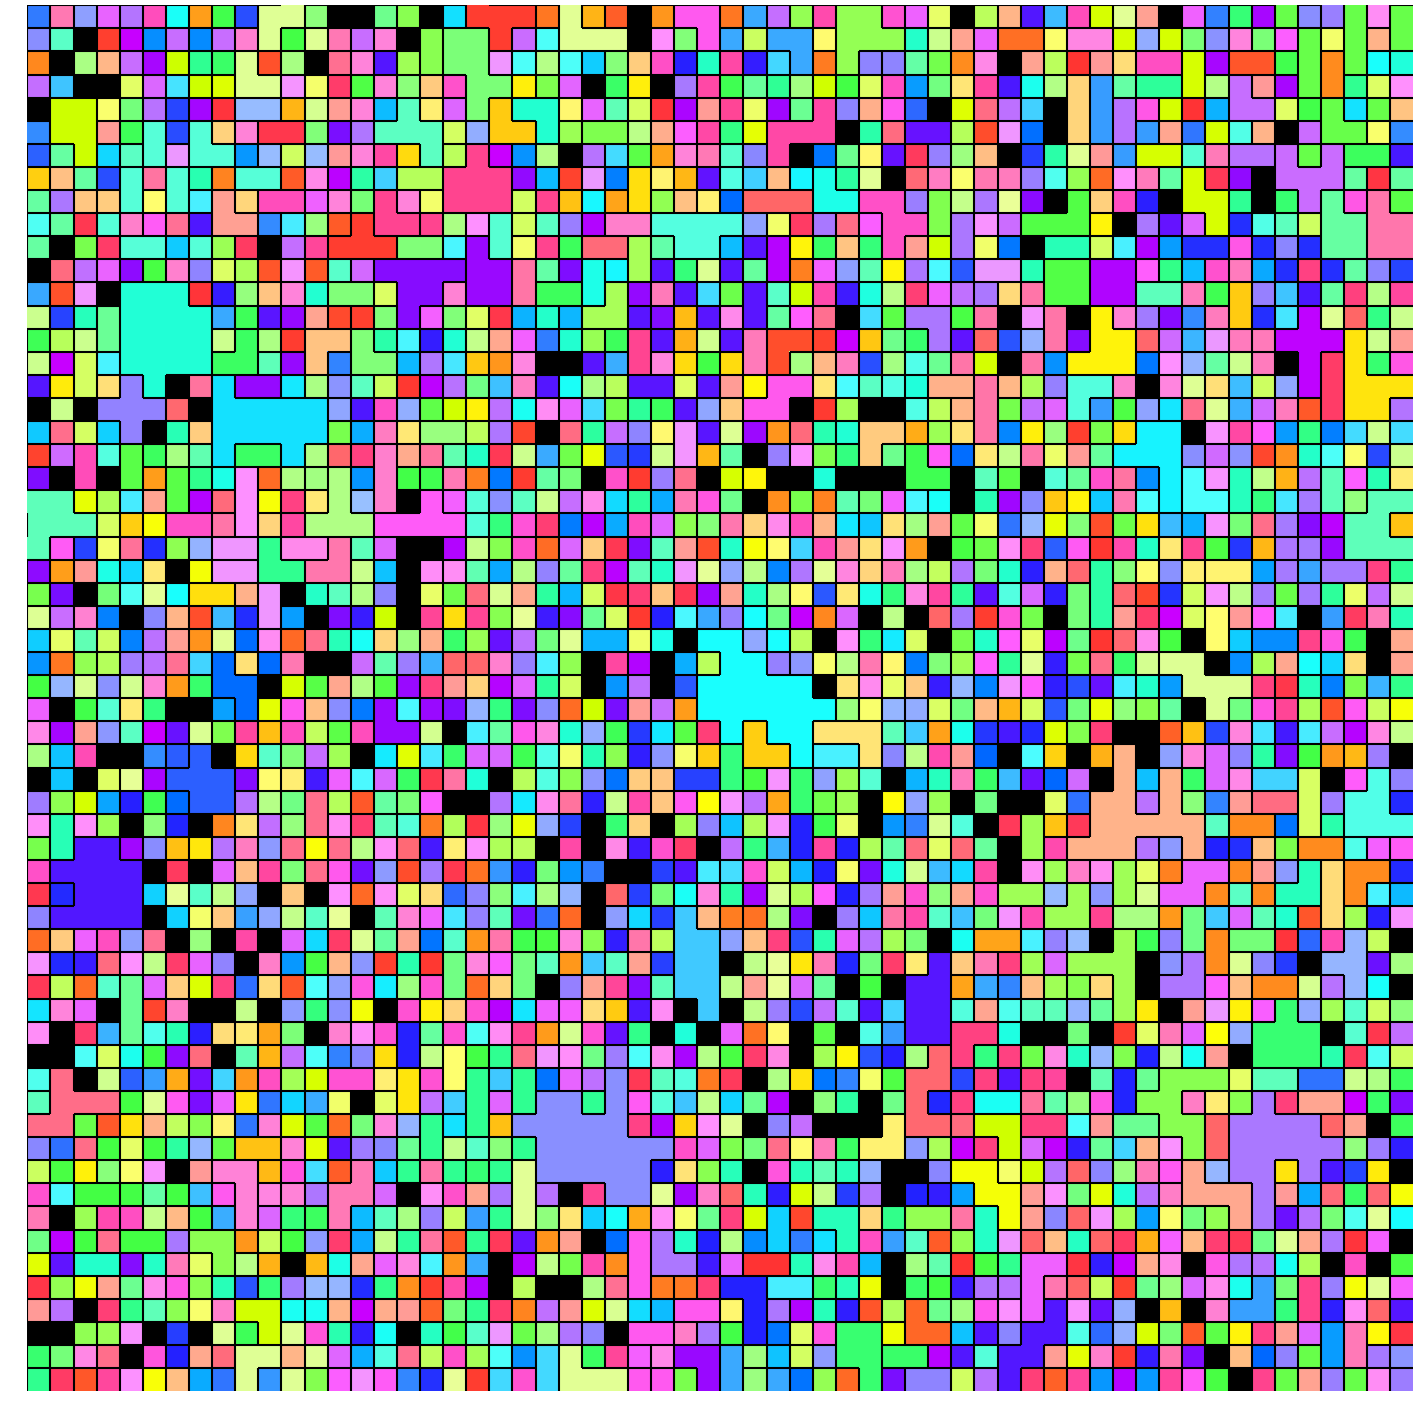
\includegraphics[width=\columnwidth]{seed=1001+title=channel_viz+treat=wave-big__mut-e_extreme+update=50000+_data_hathash_hash=6532b779898a7959+_script_fullcat_hash=474b4115ecde8750+_source_hash=d53f428-clean+ext=}
\end{subfigure}
\caption{
Representative same-channel signaling network end states for runs of each treatment.
A single cell-like organism occupies each grid tile except for black tiles, which are empty.
Channel IDs are coded by color.
Same-channel groups appear as uniformly-colored clumps, bounded by a black border.
}
\label{fig:outcome_grids}
\end{center}
\end{figure}
